\graphicspath{{4seq/asy/}}

\section{Sequences as Functions}

We've seen many different types of function in this course and used them to model various situations. In practice, one is often faced with the opposite problem: given experimental data, what type of function should you try?

\subsection{Polynomial Sequences: First, Second, and Higher Differences}

To begin to answer this, first ask yourself, ``What is a sequence?'' Hopefully you have a decent intuitive idea already. More formally, a sequence is simply a function whose domain is a set like the natural numbers, for example\par
\begin{minipage}[t]{0.6\linewidth}\vspace{-8pt}
\[f:\N\to\R:n\mapsto 3n^2-2\]
defines the sequence
\[\bigl(f(1),f(2),f(3),\ldots\bigr)=\bigl(1,10,25,46,73,\ldots\bigr)\]
Suppose instead that all you were given was a data set, say from an experiment
\[\begin{array}{c|ccccc}
x&1&2&3&4&5\\\hline
y&1&10&25&46&73
\end{array}\]
\end{minipage}\hfill\begin{minipage}[t]{0.39\linewidth}\vspace{-10pt}
\flushright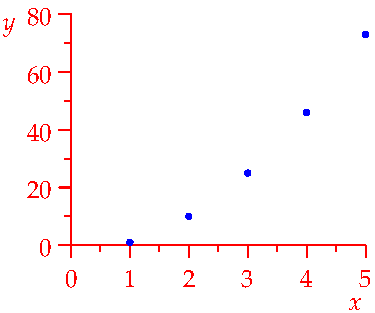
\includegraphics{seqquadex}
\end{minipage}
\bigbreak

Could you recover the original function $y=f(x)$ directly from this data? You could try several things, including plotting data points as we've done above, though it is hard to look at the plot and decide whether we should try a quadratic model, some other power function/polynomial, or perhaps an exponential. In reality, your data will have some physical interpretation which might also give you some clues.
\medbreak
Rather than guessing from a picture, a more mathematical approach involves considering how data values \emph{change} as we move along the table.
\[
	\xymatrix @R0pt @C15pt{
		x & 1 \ar@/^/[r]^{\textcolor{blue}{+1}} & 2 \ar@/^/[r]^{\textcolor{blue}{+1}} & 3 \ar@/^/[r]^{\textcolor{blue}{+1}} & 4 \ar@/^/[r]^{\textcolor{blue}{+1}} & 5\\
		y & 1 \ar@/_/[r]_{\textcolor{blue}{+9}}="a" & 10 \ar@/_/[r]_{\textcolor{blue}{+15}}="b" & 25 \ar@/_/[r]_{\textcolor{blue}{+21}}="c" & 46 \ar@/_/[r]_{\textcolor{blue}{+27}}="d" & 73
		\ar @/_/_{\textcolor{red}{+6}} "a";"b" \ar @/_/_{\textcolor{red}{+6}} "b";"c" \ar @/_/_{\textcolor{red}{+6}} "c";"d"
	}
\]
In this case the \textcolor{blue}{first-differences} in the $x$-values are constant whereas those for the $y$-values are increasing
\[\bigl(y_{n+1}-y_n\bigr)=\bigl(9,15,21,27,\ldots\bigr)\]
You likely already notice the pattern: the sequence of first-differences is increasing \emph{linearly}; it is the \emph{arithmetic sequence}
\[y_{n+1}-y_n=3+6n\]
To make this even clearer, note that the sequence of \textcolor{red}{second-differences} in the $y$-values is \emph{constant} ($+6$). These facts are huge clues that we expect a quadratic function.

\goodbreak

But why? Well we can certainly check the following directly: 
\begin{description}
  \item[Linear Model] If $f(n)=an+b$, then the sequence of first-differences is constant
  \[f(n+1)-f(n)=a\]
  \item[Quadratic Model] If $f(n)=an^2+bn+c$, then the sequence of first-differences is linear and the second-differences are constant:
  \begin{gather*}
  g(n):=f(n+1)-f(n)=2an+a+b,\qquad g(n+1)-g(n)=2a
  \end{gather*}
\end{description}
  
The relationship between these results and the \emph{derivative(s)} of the original function $f(x)$ should feel intuitive: what happens if you differentiate a quadratic twice?

\begin{example}{}{easyquadmodel}
You are given the following data set\par
\begin{minipage}[t]{0.65\linewidth}\vspace{-8pt}
\[\begin{array}{c|cccccc}
x&0&2&4&6&8&10\\\hline
y&2&16&22&20&10&-8
\end{array}\]
The $x$-values have constant first-differences while the $y$-values have constant second-differences
\begin{itemize}
  \item[]First-differences:\lstsp 14, 6, $-2$, $-10$, $-18$
  \item[]Second-differences:\lstsp $-8,-8,-8,-8$
\end{itemize}
\end{minipage}\hfill\begin{minipage}[t]{0.34\linewidth}\vspace{-10pt}
\flushright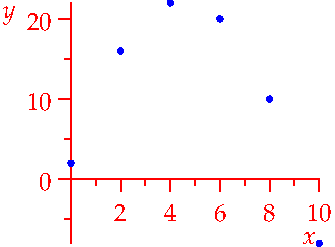
\includegraphics{seqquadex2}
\end{minipage}
\bigbreak

We therefore suspect a quadratic model $y=f(n)=an^2+bn+c$. Since the $x$-values are separated by 2 rather than 1, we should compute explicitly.\footnotemark
\begin{itemize}
  \item[]First-differences:\lstsp $f(n+2)-f(n)=a\bigl((n+2)^2-n^2\bigr)+b\bigl((n+2)-n\bigr) =4an+4a+2b$
  \item[]Second-differences:\lstsp $8a$
\end{itemize}
We conclude that $a=-1$, whence the first-differences have the form
\[f(n+2)-f(n)=-4n-4+2b\]
Taking $n=0$ quickly shows that
\[14=-4+2b\implies b=9\implies f(n)=-n^2+9n+c= -n^2+9n+2\]
where $c=2$ was also found by considering $n=0$.
\end{example}

\footnotetext{We could alternatively substitute $2x=z$ and use the above formulæ.}

There are at least two issues with our method:
\begin{enumerate}
  \item The question we're answering above is, ``Find a quadratic model satisfying this data.'' Think about why the observation of constant first-/second-differences isn't enough to \emph{guarantee} that the only model is linear/quadratic. 

  \item It is very unlikely that real experimental data will fit such precise patterns: why not? If the differences are \emph{close} to satisfying such patterns, however, then you should feel confident that a linear/quadratic model is a good choice.
\end{enumerate}
\goodbreak

\begin{example}{}{almostquadseq}
Given the data set\par
\begin{minipage}[t]{0.65\linewidth}\vspace{-10pt}
\[\begin{array}{c|cccccc}
x&0&2&4&6&8&10\\\hline
y&3&23&41&59&77&93
\end{array}\]
with sequences of first- and second-differences
\begin{itemize}
  \item[]First-differences: 20, 18, 18, 18, 16
  \item[]Second-differences: $-2$, 0, 0, $-2$ 
\end{itemize}
\end{minipage}\hfill\begin{minipage}[t]{0.34\linewidth}\vspace{-10pt}
\flushright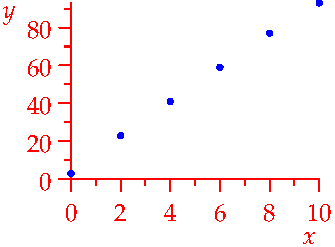
\includegraphics{seqquadex3}
\end{minipage}\smallbreak
do you think a linear or quadratic model would be superior?\smallbreak
If you wanted a linear model, you'd likely be inclined to try $f(x)=9x+b$ for some constant $b$. Here are two options:
\begin{enumerate}
  \item $f(x)=9x+5$ fits the middle four data values perfectly, but as a predictor is too large at the endpoints: $f(0)=5>3$ and $f(10)=95>93$.
  \item $f(x)=9x+5-\frac 23$ doesn't pass through any of the data values but seems to reduce the net error to zero:
  \[\def\arraystretch{1.2}\begin{array}{c|cccccc}
	x&0&2&4&6&8&10\\\hline
	f(x)-y&-\frac 43&\frac 23&\frac 23&\frac 23&\frac 23&-\frac 43
	\end{array}
	\implies \sum_x f(x)-y=0\]
\end{enumerate}
Neither model is perfect, but then this is what you expect with real-world data!
 %What happens if you ask a spreadsheet?
%f(x)\approx 3+10n-0.1n^2 rounded to nearest integer 
\end{example}

\begin{exercises}{}{}
\exstart For each data set, find a function $y=f(x)$ modelling the data.
\begin{align*}
&\text{(a)}\lstsp\begin{array}[t]{c|ccccc}
		x&2&4&6&8\\\hline
		y&-1&2&7&14
		\end{array}
&&\text{(b)}\lstsp\begin{array}[t]{c|ccccc}
		x&2&5&8&11&14\\\hline
		y&-6&-15&-6&21&66
		\end{array}
&&\text{(c)}\lstsp\begin{array}[t]{c|ccccc}
		x&0&6&9&15\\\hline
		y&3&15&21&33
		\end{array}
\end{align*}
(\emph{Be careful with (c): the $x$-differences aren't constant!})

\begin{enumerate}\setcounter{enumi}{1}  
  \item Suppose a table of data values containing $(x_0,y_0)$ has constant first-differences in both variables
  \[\Delta x=x_{n+1}-x_n=a,\quad  \Delta y=b\]
  Find the equation of the linear function $y=f(x)$ through the data.
  
%   \item Suppose data has constant $x$-differences $\Delta x=a$ and constant second $y$-differences $b$. Explain how to find the formula for the \emph{quadratic} function $y=f(x)$ passing through the data.\\
%   (\emph{Don't compute the full expression unless you're feeling masochistic!})

  \item What relationship do you expect to find with the sequential differences of a cubic function $f(n)=an^3+bn^2+cn+d$? What about a degree-$m$ polynomial $f(n)=an^m+bn^{m-1}+\cdots$?
  
  \item If $f(n)=an^2+bn+c$ is a quadratic model for the data in Example \ref{ex:almostquadseq} with constant second-differences $-1$, show that $a=-\frac 18$. What might be reasonable values for $b,c$?  
  
  \item (Hard)\lstsp Suppose $f(x)$ is a twice-differentiable function and $h>0$ is constant. Use the mean value theorem from calculus to explain the following.
  \begin{enumerate}
    \item First-differences $f(x+h)-f(x)$ are proportional to $f'(\xi)$ for some $\xi\in (x,x+h)$.
    \item Second-differences satisfy $\bigl(f(x+2h)-f(x+h)\bigr)-\bigl(f(x+h)-f(x)\bigr)=f''(\xi)h\alpha$ for some $\xi$ between $x$ and $x+h$ and some $\alpha$. Why is it unlikely that $\alpha$ is constant?
  \end{enumerate}
\end{enumerate}
\end{exercises}



\clearpage





\subsection{Exponential, Logarithmic \& Power Sequences}

To observe other relationships between data values, you might have to consider \emph{ratios} between successive terms and/or skip values to get suggestive relationships.

\begin{example}{}{}
From a first glance at the given data, it is hard to decide whether an exponential or a quadratic (or higher degree polynomial) model is more suitable. If we try to apply the constant-difference method, we don't seem to get anything helpful:\par
\begin{minipage}[t]{0.65\linewidth}\vspace{0pt}
\[
	\xymatrix @R0pt @C15pt{
		x & 1 \ar@/^/[r]^{\textcolor{blue}{+2}} & 3 \ar@/^/[r]^{\textcolor{blue}{+2}} &  5 \ar@/^/[r]^{\textcolor{blue}{+2}} & 7 \\
		y & 15 \ar@/_/[r]_{\textcolor{blue}{+120}}="a" & 135 \ar@/_/[r]_{\textcolor{blue}{+1080}}="b" & 1215 \ar@/_/[r]_{\textcolor{blue}{+9720}}="c" & 10935 
		\ar @/_/_{\textcolor{red}{+960}} "a";"b" \ar @/_/_{\textcolor{red}{+8640}} "b";"c" 
	}
\]
By the time we're looking at second-differences, any conclusion would be very weak since we only have two data values!
\end{minipage}\hfill\begin{minipage}[t]{0.34\linewidth}\vspace{-10pt}
\flushright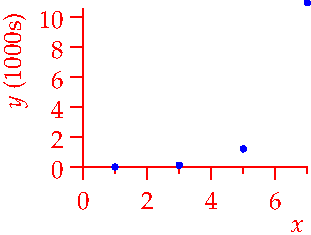
\includegraphics{seqquadex4}
\end{minipage}\medbreak

If instead we think about \emph{ratios} of $y$-values, then a different pattern emerges:
\[
	\xymatrix @R0pt @C15pt{
		x & 1 \ar@/^/[r]^{\textcolor{blue}{+2}} & 3 \ar@/^/[r]^{\textcolor{blue}{+2}} &  5 \ar@/^/[r]^{\textcolor{blue}{+2}} & 7 \\
		y & 15 \ar@/_/[r]_{\textcolor{blue}{\times 9}} & 135 \ar@/_/[r]_{\textcolor{blue}{\times 9}} & 1215 \ar@/_/[r]_{\textcolor{blue}{\times 9}} & 10935 
	}
\]
The question remains: what type of function scales its output by 9 when 2 is added to its input: $f(x+2)=9f(x)$? This is a function that converts \emph{addition} to \emph{multiplication}: an exponential! If we try $y=f(x)=ba^x$ for some constants $a,b$, then
\[f(x+2)=ba^{x+2}=ba^2b^x=a^2f(x)\]
from which a suitable model is $y=5\cdot 3^x$.
\end{example}

% \begin{example}{}{}
% If we try to apply the constant-difference method to the following data, we don't seem to get anything helpful:
% \[
% 	\xymatrix @R0pt @C15pt{
% 		x & 3 \ar@/^/[r]^{\textcolor{blue}{+3}} & 6 \ar@/^/[r]^{\textcolor{blue}{+3}} & 9 \ar@/^/[r]^{\textcolor{blue}{+3}} & 12 \\
% 		y & 135 \ar@/_/[r]_{\textcolor{blue}{+945}}="a" & 1080 \ar@/_/[r]_{\textcolor{blue}{+2565}}="b" & 3645 \ar@/_/[r]_{\textcolor{blue}{+4995}}="c" & 8640 
% 		\ar @/_/_{\textcolor{red}{+1620}} "a";"b" \ar @/_/_{\textcolor{red}{+2430}} "b";"c" 
% 	}
% \]
% Regardless, by the time we're looking at 2\nd{} differences, any conclusions will be very weak since we only have two data values!\par
% 
% If instead we think about \emph{ratios,} and skip the third data value, then a different pattern emerges:
% \[
% 	\xymatrix @R0pt @C15pt{
% 		x & 3 \ar@/^/[r]^{\textcolor{blue}{\times 2}} & 6 \ar@/^/[rr]^{\textcolor{blue}{\times 2}} & 9 & 12 \\
% 		y & 135 \ar@/_/[r]_{\textcolor{blue}{\times 8}} & 1080 \ar@/_/[rr]_{\textcolor{blue}{\times 8}}& 3645  & 8640  
% 	}
% \]
% The question remains: what type of function scales its output by 8 when its input is doubled: $f(2x)=8f(x)$? With a little thinking, you should settle on a \emph{cubic} power function; in this case $y=5x^3$ fits the data perfectly, including the skipped value $3645=5\cdot 9^3$.
% \end{example}

We can see the pattern in the example more generally:
\begin{description}
	\item[Exponential Model] If $f(x)=ba^x$, then adding a constant to $x$ results in
		\[f(x+k)=ba^{x+k}=a^kf(x)\]
		If $x$-values have constant differences ($+k$), then $y$-values will be related by a constant \emph{ratio} ($\times a^k$). You might remember this as `addition--product' or `arithmetic--geometric.'
% 	\item[Logarithms] These operate exactly as exponentials but in reverse. If $f(n)=\log_a x+b$, then \emph{multiplying} $x$ by a constant results in a constant \emph{addition/subtraction} to $y$:
% 		\[f(kx)=\log_a(kx)+b=\log_ak+\log_ax+b=\log_ak+f(x)\]
% 		This could be summarized as `product--addition.'
% 	\item[Power Functions] If $f(x)=ax^m$, then multiplying $x$ by a constant will do the same to $y$
% 		\[f(kx)=a(kx)^m=ak^mx^m=k^mf(x)\]
% 		We have a `product--product' relationship between successive terms.
\end{description}

Such a simple pattern is often disguised:
\begin{itemize}
  \item Complete data might not be given so you might have to skip some data values to see a pattern. For example, if our original data was
  \[\begin{array}[t]{c|ccccc}
		x&1&3&4&5&7\\\hline
		y&15&135&405&1215&10935
		\end{array}\]
		then the $x$-values are not in a strictly arithmetic sequence.
	\item As in Example \ref{ex:almostquadseq}, real-world/experimental data will only \emph{approximately} exhibit such patterns.
\end{itemize}
\goodbreak


\begin{example}{}{poprabbits}
A population of rabbits is measured every two months resulting in the data set
\[\begin{array}{c|cccccc}
t&0&2&4&6&8&10\\\hline
P&5&7&10&14&19&28
\end{array}\]
The data seems very close to being quadratic; consider the first and second sequences of $P$-differences
\[\Delta P=\bigl(2,3,4,5,9\bigr),\qquad \Delta\Delta P=\bigl(1,1,1,4\bigr)\]
However, the last difference doesn't fit the pattern. Instead, the fact that we expect an exponential model is buried in the experiment: the data is measuring population growth! We therefore instead consider the ratios of $P$-values:
\[
	\xymatrix @R0pt @C15pt{
		t & 0 \ar@/^/[r]^{\textcolor{blue}{+2}} & 2 \ar@/^/[r]^{\textcolor{blue}{+2}} & 4 \ar@/^/[r]^{\textcolor{blue}{+2}} & 6 \ar@/^/[r]^{\textcolor{blue}{+2}} & 8 \ar@/^/[r]^{\textcolor{blue}{+2}} & 10\\
		P & 5 \ar@/_/[r]_{\textcolor{blue}{\times 1.4}} & 7 \ar@/_/[r]_{\textcolor{blue}{\times 1.43}} & 10 \ar@/_/[r]_{\textcolor{blue}{\times 1.4}} & 14 \ar@/_/[r]_{\textcolor{blue}{\times 1.36}} & 19 \ar@/_/[r]_{\textcolor{blue}{\times 1.47}} & 28
	}
\]
The ratios are very close to being constant, whence an exponential model is suggested! To exactly match the first and last data values, we could take the model
\[P(t)\approx 5\left(\frac{28}5\right)^{\frac t{10}}\qquad \begin{array}{c|cccccc}
t&0&2&4&6&8&10\\\hline
P&5&7.057&9.960&14.057&19.839&28
\end{array}\]
Only $P(19)$ doesn't match when we take rounding to the nearest integer into account.

% 
% Since this is population growth, we expect an exponential model $P(t)=e^{mt+c}$. After taking logarithms of the population values, the data is very close to linear. Now perform a linear regression (this is much easier using a \href{http://math.uci.edu/~ndonalds/math8/rabbits.xlsx}{spreadsheet}---play with it!).\par
% 
% Ratio of $P_i$ is sequence $1.4$, $1.43$, $1.4$, $1.36$, $1.47$, so might try model with base $a=\sqrt{1.4}=1.183$: $P(t)=5(1.183)^t$. Results in
% \[\begin{array}{c|cccccc}
% t&0&2&4&6&8&10\\\hline
% P(t)&5&6.997&9.793&13.705&19.180&26.84
% \end{array}\]
% Better comes from geometric mean $aa=1.188077675$ ($P(10)=28.0168$)
\end{example}


We've seen that addition-addition corresponds to a linear model and that addition-multiplication to an exponential. There are two other natural combinations.

\begin{description}
	\item[Logarithms] These operate exactly as exponentials but in reverse. If $f(n)=\log_a x+b$, then \emph{multiplying} $x$ by a constant results in a constant \emph{addition/subtraction} to $y$:
		\[f(kx)=\log_a(kx)+b=\log_ak+\log_ax+b=\log_ak+f(x)\]
		This could be summarized as `product--addition.'
	\item[Power Functions] If $f(x)=ax^m$, then multiplying $x$ by a constant will do the same to $y$
		\[f(kx)=a(kx)^m=ak^mx^m=k^mf(x)\]
		We have a `product--product' relationship between successive terms.
\end{description}


\begin{examples}{}{}
Find the patterns in the following data and suggest a model $y=f(x)$ in each case.
\[\begin{array}[t]{c|cccc}
		x&6&18&54&162\\\hline
		y&1&2&3&4
		\end{array}
		\qquad\qquad\begin{array}[t]{c|cccc}
		x&3&6&9&12\\\hline
		y&135&1080&3645&8640
		\end{array}\]
\end{examples}

The sequential approach in this chapter is a form of \emph{discrete calculus}: using a pattern of \emph{differences} to predict the original function is similar to how we use knowledge of a derivative $f'(x)$ to find $f(x)$.

\goodbreak



\begin{exercises}{}{}
\exstart Find the patterns in the following data sets and use them to find a model $y=f(x)$.
\begin{enumerate}\setcounter{enumi}{1}
  \item[]\makebox[190pt][l]{(a)\lstsp $\begin{array}[t]{c|ccccc}
		x&0&1&2&3&4\\\hline
		y&80&120&180&270&405
  \end{array}$\hfill}
		(b)\lstsp$\begin{array}[t]{c|cccc}
		x&2&4&8&10\\\hline
		y&1&16&256&625
		\end{array}$\\[5pt]
		\makebox[190pt][l]{(c)\lstsp $\begin{array}[t]{c|ccccc}
		x&1&3&5&7&9\\\hline
		y&15&5&19&57&119
		\end{array}$\hfill}
		(d)\lstsp$\begin{array}[t]{c|ccccc}
		x&1&3&4&6\\\hline
		y&1&36&216&7776&
		\end{array}$\\[5pt]
		\makebox[190pt][l]{(e)\lstsp $\begin{array}[t]{c|ccccc}
		x&20&60&180&540\\\hline
		y&2&4&6&8
		\end{array}$\hfill}
		(f)\lstsp $\begin{array}[t]{c|ccccc}
		x&2&6&54&486&4374\\\hline
		y&2&4&8&12&16
		\end{array}$
		%y=2.5x-1
		%y=x^4/16
		%y=3x^2-17x+29
		%\frac{1/6}6^x
		%x=2\cdot 3^{y/2-1} \leftrightsquigarrow y=2+2\log_3\frac x2


	\item Take logarithms of the power relationship $y=ax^m$. What is the relationship between $\ln y$ and $\ln x$? Use this to give another reason why the inputs and outputs of power functions satisfy a `product--product' relationship.
	
	\item How does our analysis of exponential functions change if we add a constant to the model? That is, how might you recognize a sequence arising from a function $f(x)=ba^x+c$?
  
  \item Suppose $f(5)=12$ and $f(10)=18$. Find the value of $f(20)$ supposing $f(x)$ is a:
  \begin{enumerate}
    \item Linear function;
    \item Exponential function;
    \item Power function.
  \end{enumerate}
  If $f(20)=39$, which of the three \emph{models} do you think would be more appropriate?
\end{enumerate}
\end{exercises}
